\documentclass[11pt]{article}
\usepackage{fullpage}
\usepackage[authoryear,sectionbib]{natbib}
\linespread{1.618}
\usepackage[utf8]{inputenc}
\usepackage{lineno}
\usepackage{amsmath}
\usepackage{mathtools} 
\usepackage{hyperref}
\usepackage{amssymb,latexsym}
\usepackage[table]{xcolor}
\usepackage{xcolor}
\usepackage{breqn}	
\usepackage{todonotes}
\usepackage{subfig}
\usepackage{booktabs}
\usepackage{setspace}
\usepackage{placeins}
\usepackage[normalem]{ulem}
\usepackage{mathrsfs}
\newcommand{\ra}[1]{\renewcommand{\arraystretch}{#1}}

\linenumbers
\renewcommand\linenumberfont{\normalfont\small\sffamily}

%%%%%%%%%%%%%%%%%%%%%%%%%%%%%%%%%%%%%%%%%%%%%%%%%%%%%%%
\newcommand{\beginsupplement}{%
        \setcounter{table}{0}
        \renewcommand{\thetable}{S\arabic{table}}%
        \setcounter{figure}{0}
        \renewcommand{\thefigure}{S\arabic{figure}}%
     }
     
\makeatletter
\newcommand{\subalign}[1]{%
  \vcenter{%
    \Let@ \restore@math@cr \default@tag
    \baselineskip\fontdimen10 \scriptfont\tw@
    \advance\baselineskip\fontdimen12 \scriptfont\tw@
    \lineskip\thr@@\fontdimen8 \scriptfont\thr@@
    \lineskiplimit\lineskip
    \ialign{\hfil$\m@th\scriptstyle##$&$\m@th\scriptstyle{}##$\crcr
      #1\crcr
    }%
  }
}
\makeatother

\makeatletter
\newcommand{\shorteq}{%
  \settowidth{\@tempdima}{\odot}% Width of hyphen
  \resizebox{\@tempdima}{\height}{=}%
}
\makeatother

\newcommand\textequal{%
 \rule[.4ex]{4pt}{0.4pt}\llap{\rule[.7ex]{4pt}{0.4pt}}}         
%%%%%%%%%%%%%%%%%%%%%%%%%%%%%%%%%%%%%%%%%%%%%%%%%%%%%%%



\begin{document}



Yaniv\\
-more biological background in the intro\\
-don't say gamete wastage\\
-male, female instead of pollen pistil\\


\section*{Introduction}


Matings between sufficiently diverged populations or species produce low fitness hybrids, or fail altogether, due to the action of intrinsic incompatibilities(\citealt{dobzhansky1937}, citealt{muller1942}) or ecological barriers \textcolor{red}{(Schluter 1998)}. %YANIV DOUBLE CHECK THIS REFERENCE IS ABOUT ECOLOGICAL BARRIERS
  Misallocated reproductive effort spent on producing low fitness hybrids can be prevented through natural selection favoring prezygotic barriers, a process known as reinforcement \citep{Dobzhansky1937,Servedio:2003dw}.
Reinforcement is generally conceptualized as the evolution of an assortative mating locus (felsenstein1981) or female preference locus (servedioANDkirkpatrick).   
Both reinforcement mechanisms assume males and females have a shared interest in preventing the production of low-fitness hybrid offspring. 
However, reproductive interactions are generally more fractious than this, as the costs of reproductive effort can differ by sex and reproductive stage (ranging from gamete formation to mating itself) (arnqvistandrowebook).  
Because male and female interests are not always aligned, interspecific sexual conflict over the hybridization rate (parkerANDpatridge) may create an often overlooked hurdle to the evolution of reinforcement.   
We develop a population genetic model of interspecific sexual conflict and show that it prevents the long term maintenance of reinforcement.  
We suggest that interspecific sexual conflict may be particularly severe after mating, hampering the reinforcement of postmating-prezygotic reproductive isolating barriers.  

SENTENCE ABOUT REINFORCEMENT IN SYMPATRY
The process of reinforcement has gained widespread acceptance due to theoretical models showing its plausibility (CITE), lab experiments showing its evolution (CITE), and correlative studies showing its signature (CITE).  
The most compelling cases of reinforcement involve premating barriers. 
In addition to Coyne and Orr's () and other () demonstrations of enhanced behavioral isolation of sympatric Drosophila species, the reinforcement of premating barriers has been documented in numerous taxa, including damselflies (Waage 1975, 1979), Hawaiian crickets (Otte 1989), frogs (Blair 1974, Littlejohn and Loftus-Hill 1968, Hobel and Gerhardt 2003,?), fish (Rundle and Schluter 1998), birds? (Ratcliffe and Grant 1983b), Saetre et al (1997), and plants (Hopkins). %YOU WROTE: "Newer refs? These look old/classic. I have not read them all.. wonder if they show reinforcement or reproductive character displacement" I AM GOING TO LEAVE THIS FOR YOU YANIV

$MOVE TO END OF FIRST PARAGRAPH? MORE PREMATING VS POSTMATING SETUP
While standard theory does not differentiate between the reinforcement of premating  and postmating-prezygotic [i.e. gametic] barriers, ``bona fide cases of reinforcement and of gametic isolation are still rare" (Turissini et al 2017). %YANIV CAN YOU CHECK THIS QUOTE?
In fact, we know of only two unequivocal cases. 
First, the wild gingers species,  \textit{Costus scaber}, preferentially rejects  \textit{C. pulverulentus} pollen when the populations are sympatric, but not when they are allopatric (Kay and Schemske (2008)).  %pollen-pistil incompatibility, postmating prezygotic
Second, the extent of gametic isolation between \textit{Drosophila yakuba} females and \textit{D. santomea} males is stronger for sympatric than allopatric \textit{D. yakuba} samples  (Matute (2010)). 
Counter to these two examples, comparative surveys in both \textit{Drosophila} (Turissini et al 2017) and plants \citep{Moyle et al 2004} fail to find a broad signature of reinforcement of postmating-prezygotic barriers. 
There are few other plausible cases of postmating-prezygotic reinforcement in maize (cite), sea urchins (Lessios, 2007, Palumbi and Lessios 2005; Vacquier and Swanson 2011), and mussels (Slaughter et al 2008), however, these appear to involve barriers that are ineffective (Slaughter et al 2008) and/or reflect the action of selection on intraspecific matings (CITE). 

Interspecific sexual conflict could explain the difference in the frequency of reinforcement of premating and postmating-prezygotic barriers.   
Sexual conflict arises when different reproductive strategies maximize the fitness of each sex.    
 Sexual conflict in interspecific reproductive interactions can occur when the sexes `disagree' on the optimal hybridization rates \citep{Parker:1998bx}.  
The extent of this disagreement will reflect sex-specific differences in the trade-off between intraspecific and interspecific reproductive success, but is likely to be more intense for postmating barriers.
Consider the fate of a sperm (or pollen grain) in the reproductive tract of a heterospecific female. 
Without sperm limitation and with nonzero hybrid fitness, male fitness will increase and female fitness will decrease when sperm fertilize heterospecific eggs.   
In this case, selection will favor mechanisms by which male gametes overcome postmating barriers in females of other species, preventing reinforcement and breaking down reproductive isolation between species.   
By contrast, the reinforcement of pre-mating barriers may involve less conflict, because a trait preferred by conspecifics is disfavored by heterospecifics.   
Of course this distinction is not absolute --  the extent of sexual conflict will depend on how mechanistic details of premating and postmating interactions mediate the  sex-specific tradeoff between inter- and intraspecific reproductive success. 

The possibility of an interspecific sexual conflict over hybridization has been pointed out previously \citet{Parker:1998bx}, and has since been discussed briefly by \citet{Gavrilets:2005gl} and Coyne and Orr (1998).  
\citet{Parker:1998bx} modeled sexual conflict as an evolutionary game between males and females where the costs of searching for a mate could be outweighed by the benefits of siring a low fitness hybrid. 
Their model clearly highlights the potential for a sexual conflict over reinforcement, but it does not include any explicit genetics.  We therefore do not know how this conflict affects the co-evolution of male traits and female preferences, the impacts of this conflict on patterns of introgression, and the broader genomic consequences of such conflict and its resolution. 

We compare the evolution of reproductive isolation in the presence and absence of sexual conflict over hybridization. 
The mechanism for assortative mating between incipient species is modeled as two sex-limited loci, a barrier expressed in female gametes and a compatibility allele expressed in male gametes.  
Reproductive isolation evolves to completion when there is no sexual conflict, but is only transient  when sexual conflict selects for males to overcome the barrier in the other species.  
As we elaborate in the discussion, transient evolution of reinforcement in the face of sexual conflict is broadly consistent with numerous empirical observations, including patterns of reproductive isolation between hybridizing \textit{Z. mays} subspecies.  
Overall, we find that sexual conflict is a potentially important force breaking down reinforcement or hindering the evolution of isolating barriers between species. 


\section*{Modeling}

We built a population genetic model to examine the role of sexual conflict in breaking down reinforcement. We assume two previously allopatric populations have diverged at a local adaptation locus and male compatibility locus. Upon secondary contact, the populations exchange migrants and form maladaptive hybrids, creating selection for the evolution of a female barrier. We are interested in the evolution of reproductive isolation in a focal population. There are three loci relevant to our focal population, all on the same chromosome: the female barrier locus, the male compatibility locus, and the local adaptation locus. 

Viability selection operates at the local adaptation locus \textbf{L}. The \emph{L} allele is adaptive in population one and the \emph{$\ell$} allele is adaptive in population two; both alleles are initially fixed in the population in which they are favoured. Maladaptive alleles are selected against with selection strength $s_n$ in population $n$.  Selection acts multiplicatively. For example, hybrid offspring heterozygous at the local adaptation locus($L \ell$) experience a selection strength of $(1-s_n)$ while maladaptive homozygotes experience a selection strength of $(1-s_n)^2$. This ecological divergence gives rise to postzygotic (ecological) isolation between population one and population two that can be reinforced by assortative mating.

Assortative mating between these (incipient) species is governed by a female locus, \textbf{F}, expressed in female gametes, and a male compatibility locus, \textbf{M}, expressed in male gametes.  Females with the barrier allele, \emph{F}, block fertilization by males without the male compatibility allele, \emph{M} (Fig. \ref{fig:model}B).  Females with the alternative allele, \emph{f}, can be fertilized by males carrying either \emph{M} or \emph{m}.  We assume that the barrier allele is initially rare in our focal population and absent in the non-focal population. Each generation begins with migration of haploid males.  Formation of diploid zygotes is governed by the assortative mating loci.  Diploid offspring undergo viability selection before forming haploid gametes via meiosis (involving both recombination and segregation). We track the change in genotype frequencies after each generation to understand the evolution of reproductive isolation.

While we describe $F$ as the `barrier' allele throughout, it is important to note that $F$ is only an effective barrier to hybridization if the compatibility allele ($M$) is not common in the other species.  Therefore, reproductive isolation is measured as the fraction of heterospecific males that are rejected (\emph{Methods}, equation \ref{Eq:eq4}. Reinforcement is considered complete (equals one) when all heterospecific males are rejected.  This definition is useful for understanding the short- and long-term consequences of sexual conflict on the evolution of reproductive isolation. 

Sexual conflict over hybridization arises between females and the fraction of males in the mating pool that are migrants.  Males that have migrated will be selected to hybridize in order to avoid associated opportunity costs, while females will be selected to avoid making unfit hybrid offspring, preferring conspecific males.  To measure the extent of the conflict we calculated female and migrated male fitness relative to their respective optimum fitness.  Female fitness is calculated as the absolute fitness (after mating and selection) of all diploid offspring in a population.  Optimum female fitness is the absolute fitness of diploid offspring if all heterospecific male gametes are rejected.  It is important to emphasize that optimum fitness will not always be one, but varies from generation to generation with the frequency of maladaptive alleles in the population.  Because the conflict is between resident females and \emph{immigrant} males, migrant male fitness is defined as the absolute fitness of only the diploid offspring sired by heterospecific males.  Optimum migrant male fitness is the absolute fitness if all immigrant males fertilized females (in terms of the conflict, males would have no fitness if all immigrant males were rejected).  Similar to optimum female fitness, optimum migrant male fitness varies with local adaptation allele frequency. Rigorously defining the conflict in this manner helps us understand the evolutionary forces driving or hindering reproductive isolation. It also allows us to design a model without sexual conflict.

We compare our model to one without sexual conflict by using a premating barrier instead of a postmating prezygotic barrier.  The key aspect of the premating model is that migrated males rejected by heterospecific females have the opportunity to `return' to their native population and fertilize conspecific females.  \textcolor{red}{EMPIRICAL EXAMPLES pollinator behaviour, flowering time, reproductive cycle (sea urchins), animals -> rejected by females and search until the find a mate that accepts them \textcolor{red}{Levin (1978), Grant (1994) from Moyle et al (2004)}}. Male and female interests are aligned because males that are rejected by heterospecific females (and therefore do not hybridize) have higher fitness than males that do hybridize by overcoming the premating isolating barrier.  We model this premating barrier by assuming that the migration rate is genotype dependent.  For example, $M f \ell$ male gametes will always have $\eta[i_1 i_2] = \eta_{max}$ whereas $M f \ell$ gametes will only have $\eta[i_1 i_2] = \eta_{max}$ if there is no barrier in the focal population, and $\eta[i_1 i_2] < \eta_{max}$ otherwise.  

Up to this point, we have described the model from the perspective of the focal population and assumed there is one potential isolating barrier. Based on the mechanism of assortative mating, the barrier can only prevent hybridization in one direction. (If the barrier allele were to increase in frequency in the non-focal population, it would offer no reproductive isolation because the corresponding compatibility allele is initially fixed, and remains common, in the focal population). This formulation does not allow the evolution of reproductive isolation in the non-focal population, potentially facilitating the spread of the compatibility allele from population one to population two. 

To avoid the flow of genes (i.e., $M$) that break down reproductive isolation, we assume the non-focal population has it own set of assortative mating loci and a second local adaptation locus (found together on a separate chromosome to the original three loci). Initial conditions are chosen such that our focal species will evolve an isolating barrier through locus \textbf{\texorpdfstring{F\textsubscript{1}}{F 1}} and species two through locus \textbf{\texorpdfstring{F\textsubscript{2}}{F 2}}. Specifically, in population one we assume that at the first set of assortative mating loci, the compatibility allele ($M_1$) is fixed and the barrier is rare ($p_{F_1} = 0.05$). At the other set of assortative mating loci, the compatibility allele ($M_2$) is absent and males could not overcome an isolating barrier in the other species if the barrier were common.  Initial genotype frequencies in population two are analogous (i.e., $M_2$ is fixed and $F_2$ is rare, while males could not overcome an isolating barrier in population one). Selection acts multiplicatively within and between loci to determine the overall strength of selection.  

We track haploid genotype frequencies using forward iterations of the recursion equations described in the \emph{Methods}.  With a total of six loci and 64 haploid genotypes in each species, the equations are sufficiently complicated that we could not obtain analytical solutions.  Furthermore, because the evolution of reinforcement is transient (see Fig. \ref{fig:sample}C), we are interested in the short-term dynamics of the system instead of long-term equilibria.  


\begin{figure}[!htb]
\centering
\subfloat{\label{fig:figure1}
\includegraphics[width=1.0\textwidth]{figure1All.pdf}}
%\subfloat{\label{fig:table1}
%\includegraphics[width=0.3\textwidth]{table1.pdf}}
\caption{(A) Model of postmating prezygotic isolation between two populations. Alleles shown at each locus are initially fixed unless the alternative (rare) allele is indicated in red. Species one has $f_1$ at high frequency and a rare barrier, $F_1$.  Initially, most males from species two can fertilize species one females, selecting for an increase in the frequency of the $F1$ allele to avoid the production of low fitness hybrid offspring.  Similarly, most migrated males from species one can initially fertilize species two females. We investigate whether reinforcement evolves or whether $M_2$ and $M_1$, in species one and two, respectively, spread to prevent the evolution of isolating barriers that complete speciation. (B) Table describing assortative mating based on loci \textbf{\texorpdfstring{F\textsubscript{1}}{F 1}} and \textbf{\texorpdfstring{F\textsubscript{2}}{F 2}}, expressed in females, and loci \textbf{\texorpdfstring{M\textsubscript{1}}{M 1}} and \textbf{\texorpdfstring{M\textsubscript{2}}{M 2}}, expressed in males.  $M_1$ males can fertilize $F_1$ and $f_1$ females, while $m_1$ males can only fertilize $f_1$ females. Assortative mating works analogously with respect to the \textbf{\texorpdfstring{F\textsubscript{2}}{F 2}} and \textbf{\texorpdfstring{M\textsubscript{2}}{M 2}} loci. The two sets of assortative mating loci act additively, i.e., an $M_1 m_2$ male could not fertilize an $F_1 F_2$ female. }
\label{fig:model}
\end{figure}



%%%%%%%%%%%%%%%%%%%%%%%%%%%%%
\section*{Results}

We compare a model with sexual conflict (where the barrier is postmating prezygotic) to one without (where the barrier is premating) with the goal of understanding how sexual conflict over the hybridization rate affects the evolution of reproductive isolation. Forward recursions were carried out across a range of parameter values. 

\subsection*{Evolution of Reproductive Isolation is Transient when there is Sexual Conflict}

\paragraph{Postmating prezygotic barrier:} Permanent reproductive isolation never evolves when there is sexual conflict over reinforcement, \textcolor{blue}{so long as heterozygpotes at the local adaptation locus are viable}.  
There are two ways in which the reinforcement of postmating prezygotic barrier fails. 
First, if divergent selection selection is sufficiently weak and recombination is sufficiently strong, the female barrier fails to increase in frequency (see below).
Alternatively, if divergent selection is sufficiently strong and recombination is sufficiently weak, the initially rare female barrier allele increases in frequency in the focal population, but is ultimately undermined by the spread of the pollen compatibility allele in the other. 

We present the dynamics of this transient evolution of postmating prezygotic reinforcement for a single parameter set in Figure (Fig. \ref{fig:sample}A-B). 
The evolutionary dynamics are best understood in three phases, which we denote by shading. 
In the first phase,  the female incompatibility allele, $F$, rapidly increases in frequency in population one (\textcolor{blue}{blue line} in Fig. \ref{fig:sample}A) because it prevents fertilization by migrants (heterospecifics), and therefore does not produce maladapted hybrid offspring.   
While this postmating prezygotic barrier spreads quickly in population one, it is initially disfavored in population two because it would result in preferential mating with heterospecifics.  
As such, haplotypes bearing the $F$ allele do not initially increase in frequency in population two (note the absence of XXX in Fig. \ref{fig:sample}B). 
However, as the $F$ allele increases in frequency in population one, migrant compatible male gametes  (i.e. haplotypes with $M$ alleles) have higher fitness than incompatible male gametes because they can gain some reproductive success from mating with incompatible females.  
Thus, in the second phase, the  $Mf\ell$ haplotype rapidly increases in frequency in population two (orange line Fig. \ref{fig:sample}B), as it is locally adapted, does not reject $m$ male gametes, but can fertilize $F$ females. 
Once the $M$ allele is sufficiently common in both populations, $F$ is both ineffective at preventing heterospecific matings in population one, and does result in preferential matings with heterospecifics in population two. 
Therefore in the third phase, the frequency of $F$ slowly homogenizes across populations by migration (Fig. \ref{fig:sample}A-B).
The level of reproductive isolation thus reaches a maximum before evolving towards zero (Fig. \ref{fig:sample})C.  
While figures \ref{fig:sample}A-D show a single parameter combination, this result is qualitatively consistent over all parameter combinations that allow for the initial spread of a postmating prezygotic barrier to prevent the production of hybrids. 



\paragraph{Premating barrier:} In comparison, without sexual conflict, full reproductive isolation evolves over a wide range of parameter space.  
The key aspect of the premating model that facilitates the evolution of reinforcement is that rejected migrant male gametes have the opportunity to fertilize conspecifics.   
We present the dynamics of the successful evolution of premating reinforcement for a single parameter set in Figure (Fig. \ref{fig:sample}E-H). 
As in the postmating model, the female barrier $F$, increases in frequency in population one because the barrier allele initially prevents costly hybridization (Fig. \ref{fig:sample}E). 
However, different dynamics occur in population two. 
%rare $M$-carrying migrant males mate with and fertilize any type of heterospecific female (regardless of the allele at the \textbf{F} locus). 
This is because, unlike the postmating model,  $m$-carrying migrant males that are rejected (by $MFL$ females in population one), return to population two where they fertilize conspecific females and have higher fitness than hybridizing $M$-carrying males.  
Thus, the $m$ allele remains at high frequency in population two (Fig. \ref{fig:sample}F) and reproductive isolation evolves between the two populations (Fig. \ref{fig:sample}G).  
While Figs. \ref{fig:sample}E-H show a characteristic trajectory for the reinforcement of premating barriers, this outcome is not universal. 
As we show below, weak selection against hybrids and/or high recombination rates between loci lead to transient reinforcement, however the dynamics of this case differ substantially from that of the postmating prezygotic barrier. 

To illustrate the sexual conflict over reinforcement, we plot male and female fitness relative to their respective optima (Fig. \ref{fig:sample}D and H). 
In the postmating prezygotic model, female fitness is maximized when reproductive isolation is maximized (Fig. \ref{fig:sample}D). 
This coincides with the time at which migrated male gametes is lowest; the male compatibility allele is still at low frequency in population two and most migrated male gametes are rejected.  
However, at equilibrium, male fitness equals optimum male fitness (such that relative fitness is one) because the $M$ allele is fixed and migrant males can fertilize any type of heterospecific female. 
We note that this does not mean that migrated males that hybridize have higher fitness than males that remain in their own population and mate with conspecifics migrated males have the highest fitness possible, given that they have mated with heterospecifics. 
Relative female fitness is less than one at equilibrium because a fraction $\eta_{21}/((1-\eta_{12} + \eta_{21})$ of females are fertilized by migrant (heterospecific) males. \textcolor{red}{TURN THE EQUATION INTO WORDS}.
In comparison with the postmating model, male and female fitness in the premating model are both equal to their respective fitness optima at equilibrium (Fig. \ref{fig:sample}H).  
When there is reproductive isolation between the two populations, all migrated males are rejected by heterospecific females.  
This is optimal for females and for potentially hybridizing males (those that are relevant to the conflict) because rejected males have higher fitness mating with conspecifics.

\subsection*{High gene flow prevents the evolution of reproductive isolation}\label{section:migration}

\paragraph{Postmating prezygotic barrier:} So long as the migration rates between populations $i$ and $j$ ($\eta_{{i,j}}$) are both non-zero, sexual conflict always leads to transient reinforcement.  
This is apparent in Fig. \ref{fig:migration}A , as the equilibrium level of reinforcement (bottom of shaded regions) goes to zero for all migration rates. 
Migration rates do, however, alter both the transient dynamics of the evolution of reinforcement and the maximum effectiveness of the isolating barrier.  
For example, intermediate migration rates select for higher maximum levels of reproductive isolation than low or high migration rates. 
This can be seen for the case of symmetric migration (blue lines, Fig. \ref{fig:migration}A), as the maximal strength of reinforcement is greater for migration rates between 0.05 and 0.25, than it is for migration rates outside of this range.  
The evolution of reproductive isolation is limited at low migration mates because fewer maladapted hybrids are formed, exerting weaker selection on the postmating prezygotic barrier. 
In contrast, high migration rates strongly favor the postmating prezygotic female barrier, but also increase the rate at which compatible male gametes siring surviving hybrids return to population two and promote fixation of the compatible male gamete.  
This decreases the number of generations where the barrier is effective (not shown).  \textcolor{red}{WE NEED A (SUPP) FIGURE  TO BACK THIS UP.}

 Asymmetric migration rates (\textcolor{red}{red} and black lines in Fig. \ref{fig:migration}A) give further insight into the reinforcement dynamics by isolating the effect of changing migration in one direction. 
In this case, it is useful to talk about the results from the perspective of a focal population (e.g., population one, but the results are analogous for population two if chosen as the focal population). 
Higher migration rates out of population one (i.e., high $\eta_{12}$) reduce the maximal level of reinforcement by increasing the rate of migration of compatible male gametes ($M$ alleles) to population two.  
When $M$  spreads quickly into population two, it reduces the maximum level of reinforcement that evolves before it fixes and the barrier in population one is ineffective (compare the black line ($m_{12}  = 0.5$) in Fig. \ref{fig:migration}A to the red line ($m_{12} = 0.1$)). 
In comparison, increasing migration into population one (i.e., increasing $m_{21}$) allows for a higher maximum level of reinforcement (unless $m_{12}$ is also high) because the formation of many hybrids strongly favours the barrier. 

\paragraph{Premating barrier:} When selection is strong and recombination is weak, reinforcement of premating isolation is successful, and migration rates do not strongly affect the maximal levels maximal or equilibrial level of reinforcement (all lines quickly approach complete reinforcement in Fig. \ref{fig:migration}B).     
They do however, affect the rate that complete reinforcement is achieved, because realized migration rates in the premating model vary over time with genotype frequency \textcolor{red}{SUPP FIGURE MUST SHOW THIS}.  
Ignoring barrier effects on the second chromosome (for ease of understanding), $M$-carrying males will migrate at $m_{21\text{max}}$ regardless of the frequency of the barrier in population one.
$m$-carrying males will migrate at a rate close to $\eta_{21\text{max}}$ when the barrier is rare, but will effectively not migrate when the barrier is fixed. 
Selection for the barrier is therefore strongest when it is rare and decreases when the barrier is common. 
Thus, higher maximum migration rates select for a rapid increase in the barrier, while lower maximum migration rates select for slow sustained increases in the barrier, both resulting in fixation and 100\% reproductive isolation at equilibrium.   

\subsection*{Selection}\label{section:selection}
Increasing selection against maladapted genotypes (in either population) increases selection for the female isolating barrier. 

\paragraph{Postmating prezygotic barrier:} In the postmating model, we observe higher maximum levels of reinforcement before the barrier is rendered ineffective by the fixation of the male compatibility allele in the non-focal population (Fig. \ref{fig:selection}A).  
Moreover, a postmating female barrier fails to evolve altogether when selection is sufficiently weak (e.g. $s_1 = 0.1$ for the parameters in Fig. \ref{fig:selection}A).

\paragraph{Premating barrier:} The complete reinforcement of a premating barrier evolves when selection against hybrids is strong in both populations (Fig. \ref{fig:selection}B).  
Weak selection, however, can lead to transient reinforcement.  
Weak selection against hybrids in the focal population (population one) does not exert strong enough selection pressure on the barrier to increase in frequency (e.g. see the straigth grey line for $s_1 = 0.1$ for the parameters in Fig. \ref{fig:selection}B). 

Less intuitively, weak selection in population two can prevent reinforcement even when selection is very strong in population one (gray lines, Fig. \ref{fig:selection}B).  
This phenomenon requires us to simultaneously consider the barriers on chromosomes one and two, which we denote with subscripts following haplotype. 
Hybrid offspring in population two survive at relatively high rates when selection is weak (e.g., $s_2 = 0.1$ in Fig. \ref{fig:selection}\textcolor{red}{B}).  
These hybrids are either $MfL_2$ male gametes (that can fertilize any female in population two) or $mfL_2$ male gametes (that can fertilize most females in population two when the barrier $F_2$ is rare). 
Both carry the $M_1$ allele because it is fixed in population one. 
$M_1$ spreads in population two despite the fitness advantage of $m_1$-carrying males in the premating model.  
The rapid spread of the $M$ allele prevents the barrier from reaching high frequency in the focal population and makes it ineffective at preventing hybridization with population two in the long term.   
We note that while this results in the transient evolution of reinforcement, this breakdown is conceptually similar to that discovered by Servedio and Burger (2014), where a migration of foreign female preference alleles favors the invasion of the foreign male trait, rather than the postmating prezygotic conflict model, above. 

\subsection*{Recombination}\label{section:recomb}
\textcolor{red}{I somehow need to indicate on the figure which lines belong to the MFL model and which to the FML model}

Recombination is a well-recognized hurdle to the evolution of species boundaries because assortative mating loci must be associated with adaptive combinations of loci or locally adapted loci to ensure beneficial mate discrimination. Consistent with previous results, we find that recombination can prevent or limit the evolution of reproductive isolation. The extent to which it does so depends on the ordering of loci and the model (postmating versus premating).  \sout{In general, linkage between $M$ and $L$ is more important for reinforcement in the postmating model, while linkage between $F$ and $L$ is more important in the premating model.  }
%Thus, recombination rates have different consequences for the two models depending on the order of the loci ($MFL$ versus $FML$). 

\subsubsection*{Postmating}

The initially rare barrier, expressed in females, relies on the genetic association between \textbf{M} and \textbf{L} across populations to ensure accepting $M$-carrying male gametes means offspring will have the local adaptation allele. Using $M$ as an indicator of conspecifics is effective until the compatibility allele increases in frequency in the non-focal population, which occurs via three mechanisms. Initially, $M_1$ is introduced into population two by migration and hybridization; \textit{\texorpdfstring{MfL\textsubscript{1}}{MfL 1}} (or \textit{\texorpdfstring{fML\textsubscript{1}}{fML 1}}) males fertilize females ($mf\ell_1$ or $fm\ell_1$) in population two. The chromosome one male compatibility allele ($M_1$) can become associated with \textcolor{red}{the locally adapted in population two}$\ell$ in population two via recombination. Higher recombination rates facilitate introgression of the male compatibility allele onto the population two genetic background. Once present in population two, it can also increase in frequency via hybridization and subsequent back migration. Finally, recombination can give rise to genotypes carrying the barrier  and the population two local adaptation allele (i.e., $F$ and $\ell$). Once created, these $F$-carrying genotypes directly select for the compatibility allele in population two by giving it a reproductive advantage with conspecific females. \sout{If not continuously created while the compatibility allele is still spreading, genotypes carrying the barrier will disappear because \textcolor{red}{there is no selective advantage in population two.} } INCLUDE THIS LAST PART?

\textcolor{red}{Make distinction between sexual conflict mechanisms and intraspecific reproductive advantage}
The strength of the genetic association between \textbf{M} and \textbf{L} across populations depends on recombination rates and the order of the loci. Presented here are the results for loci found in the order \textbf{MFL}. Results for loci found in the order \textbf{FML} are presented in the supplementary material.
 When \textbf{F} and \textbf{L} are adjacent and tightly linked (Fig. \ref{fig:recombination}C black line), reproductive isolation evolves to higher maximums than if there is free recombination between them (Fig. \ref{fig:recombination}C grey line \textcolor{red}{flat line}). The maximum is determined by the rate of spread of the compatibility allele $M$. The compatibility allele $M$ spreads more quickly in population two when $F$ and $L$ are unlinked because this allows the barrier to \textcolor{red}{break its association with $L$ and then selected for} become associated with $\ell$. A barrier on the population two genetic background is not selected against and gives the compatibility allele a reproductive advantage within population two. In this case, the recombination rate between \textbf{M} and \textbf{F} does not significantly change the dynamics. 

In comparison, when \textbf{F} and \textbf{L} are tightly linked, maximum reproductive isolation is modulated by $r_{MF}$ (Fig. \ref{fig:recombination}C black line). Low recombination rate $r_{MF}$ limits the spread of the compatibility allele to hybridization and back migration of rarely formed $Mf\ell$ genotypes. High $r_{MF}$ facilitates the spread of the compatibility allele by regularly creating new $Mf\ell$ genotypes. Changing the order of the loci does not qualitatively effect the evolution of reproductive isolation (Fig. \ref{fig:recombination}D)
%%Re-write to be all about the genetic association between $M$ and $L$

\subsubsection*{Premating}

In the premating model, whether reproductive isolation evolves to completion depends on whether the barrier introgresses into population two. Recall that as the barrier increases in frequency in population one, only $M$-carrying males from population two can successfully mate with heterospecifics.  $m$-carrying males effectively `return' to their home population and mate with conspecific $mf\ell$ females. If \textbf{F} and \textbf{L} are tightly linked, reinforcement evolves as the barrier increases in frequency in population one while the compatibility allele decreases in frequency in population two because $m$-carrying males have higher fitness than $M$-carrying males. However, if \textbf{F} and \textbf{L} are not tightly linked, the barrier can easily recombine onto the population two genetic background. Once the barrier is present in population two, the compatibility allele has a reproductive advantage with conspecific females that allows it to spread to fixation. 

Linkage between \textbf{F} and \textbf{L} depends on recombination rates and the order of the loci. If \textbf{F} and \textbf{L} are adjacent and tightly linked, permanent reproductive isolation evolves (Fig. \ref{fig:recombination}A black line). In contrast, free recombination between \textbf{F} and \textbf{L} allows the barrier to become associated with the population two local adaption allele (Fig. \ref{fig:recombination}A grey line), which gives the compatibility allele the intraspecific reproductive advantage necessary to spread. Note that it is introgression of the barrier, not sexual conflict, that prevents the evolution of reinforcement in the premating model (similar to Servedio and Burger 2014).  If \textbf{M} and \textbf{L} are adjacent, introgression of the barrier is facilitated by increased genetic distance between $F$ and $L$. Permanent reproductive isolation is only possible if $F$ is tightly linked to $L$ through $M$. Thus, even if the compatibility and local adaptation allele are strongly linked, free recombination between $F$ and $M$ allows the barrier to recombine with $-M\ell$ to create $FM\ell$ genotypes in population two (Fig. \ref{fig:recombination}B blue line). Any recombination between $M$ and $L$ further unlinks the barrier from the local adaptation allele.


%%%%%%%%%%%%%%%%%%%%%%%%%%%%%
\section*{Results}

We compare a model with sexual conflict (where the barrier is postmating prezygotic) to one without (where the barrier is premating) with the goal of understanding how sexual conflict over the hybridization rate affects the evolution of reproductive isolation. Forward recursions were carried out across a range of parameter values. 

\subsection*{Evolution of Reproductive Isolation is Transient when there is Sexual Conflict}

\textcolor{red}{Permanent} reproductive isolation never evolves when there is sexual conflict over the hybridization rate. An initially rare barrier increases in frequency upon exchanging migrants with a closely related species.  This increase temporarily provides reproductive isolation before the barrier allele is rendered ineffective by the spread of the break allele in the other population. Genotype frequency dynamics for a sample simulation are shown in Figure \ref{fig:sample}A-B. In the focal population (population one), $MFL$ has a selective advantage because carriers of the barrier allele avoid fertilization by heterospecifics (Fig. \ref{fig:sample}A).  As the barrier increases in frequency, $M$-carrying migrant males (from population two) have a reproductive advantage over the initially more prevalent $m$-carrying migrant males. Thus, most hybrid offspring in population one carry the $Mf\ell$ genotype.  The break allele increases in frequency in population two as $Mf\ell$ genotypes introgress in subsequent generations (Fig. \ref{fig:sample}B). Once the break allele is fixed in population two, the isolating barrier in population one is no longer effective and starts declining towards its migration-selection balance equilibrium frequency.  The level of reproductive isolation thus reaches a maximum before evolving towards zero (Fig. \ref{fig:sample})C.  

In comparison, when there is no sexual conflict, full reproductive isolation evolves over a wide range of parameter space.  The key aspect of the premating model that facilitates the evolution of reinforcement is that rejected migrant males have the opportunity to mate with conspecific females.  As in the postmating model, $MFL$ increases in frequency because the barrier allele initially prevents costly hybridization (Fig. \ref{fig:sample}E). However, rare $M$-carrying migrant males mate with and fertilize any type of heterospecific female (regardless of the allele at the \textbf{F} locus). Unlike the postmating model, the fraction of $m$-carrying migrant males that are rejected (by $MFL$ females), return to population two where they fertilize conspecific females and have higher fitness than hybridizing $M$-carrying males.  Thus, the $m$ allele remains at high frequency in population two (Fig. \ref{fig:sample}F) and reproductive isolation evolves between the two populations (Fig. \ref{fig:sample}G).  While Figure \ref{fig:sample}E-H show a common outcome for the evolution of reinforcement in the premating model, reproductive isolation does not always persist at equilibrium. Weak selection against hybrids and/or high recombination rates between loci lead to transient reinforcement and is discussed further below. 

To illustrate the sexual conflict over hybridization, we also plot male and female fitness relative to their respective optima (Fig. \ref{fig:sample}D and H). In the postmating model, female fitness is maximized when reproductive isolation is maximized (Fig. \ref{fig:sample}D). This is also when the fitness of migrated males is lowest; the break allele is still at low frequency in population two and most migrated males are rejected.  At equilibrium, male fitness equals optimum male fitness (such that relative fitness is one) because the break allele is fixed and migrant males can fertilize any type of heterospecific female. It is important to note that this does not mean that migrated males that hybridize have higher fitness than males that remain in their own population and mate with conspecifics; migrated males have the highest fitness possible, given that they have mated with heterospecifics.  Relative female fitness is less than one at equilibrium because a fraction $\eta_{21}/((1-\eta_{12} + \eta_{21})$ of females are fertilized by migrant (heterospecific) males. In comparison with the postmating model, male and female fitness in the premating model are both equal to their respective fitness optima at equilibrium (Fig. \ref{fig:sample}H).  When there is reproductive isolation between the two populations, all migrated males are rejected by heterospecific females.  This is optimal for females and for potentially hybridizing males (those that are relevant to the conflict) because rejected males have higher fitness mating with conspecifics.

%- F2 acts a barrier in pop 2, and pop 2 males can overcome it
%-but have b= 0 for F1 in pop 2
%-goes over and comes back
%-what if it can't come back?

%compare to no barrier in one pop, does M spread by migration
%-does barrier spread because M can fertilize it
\begin{figure}
[!htb]
\centering
\subfloat{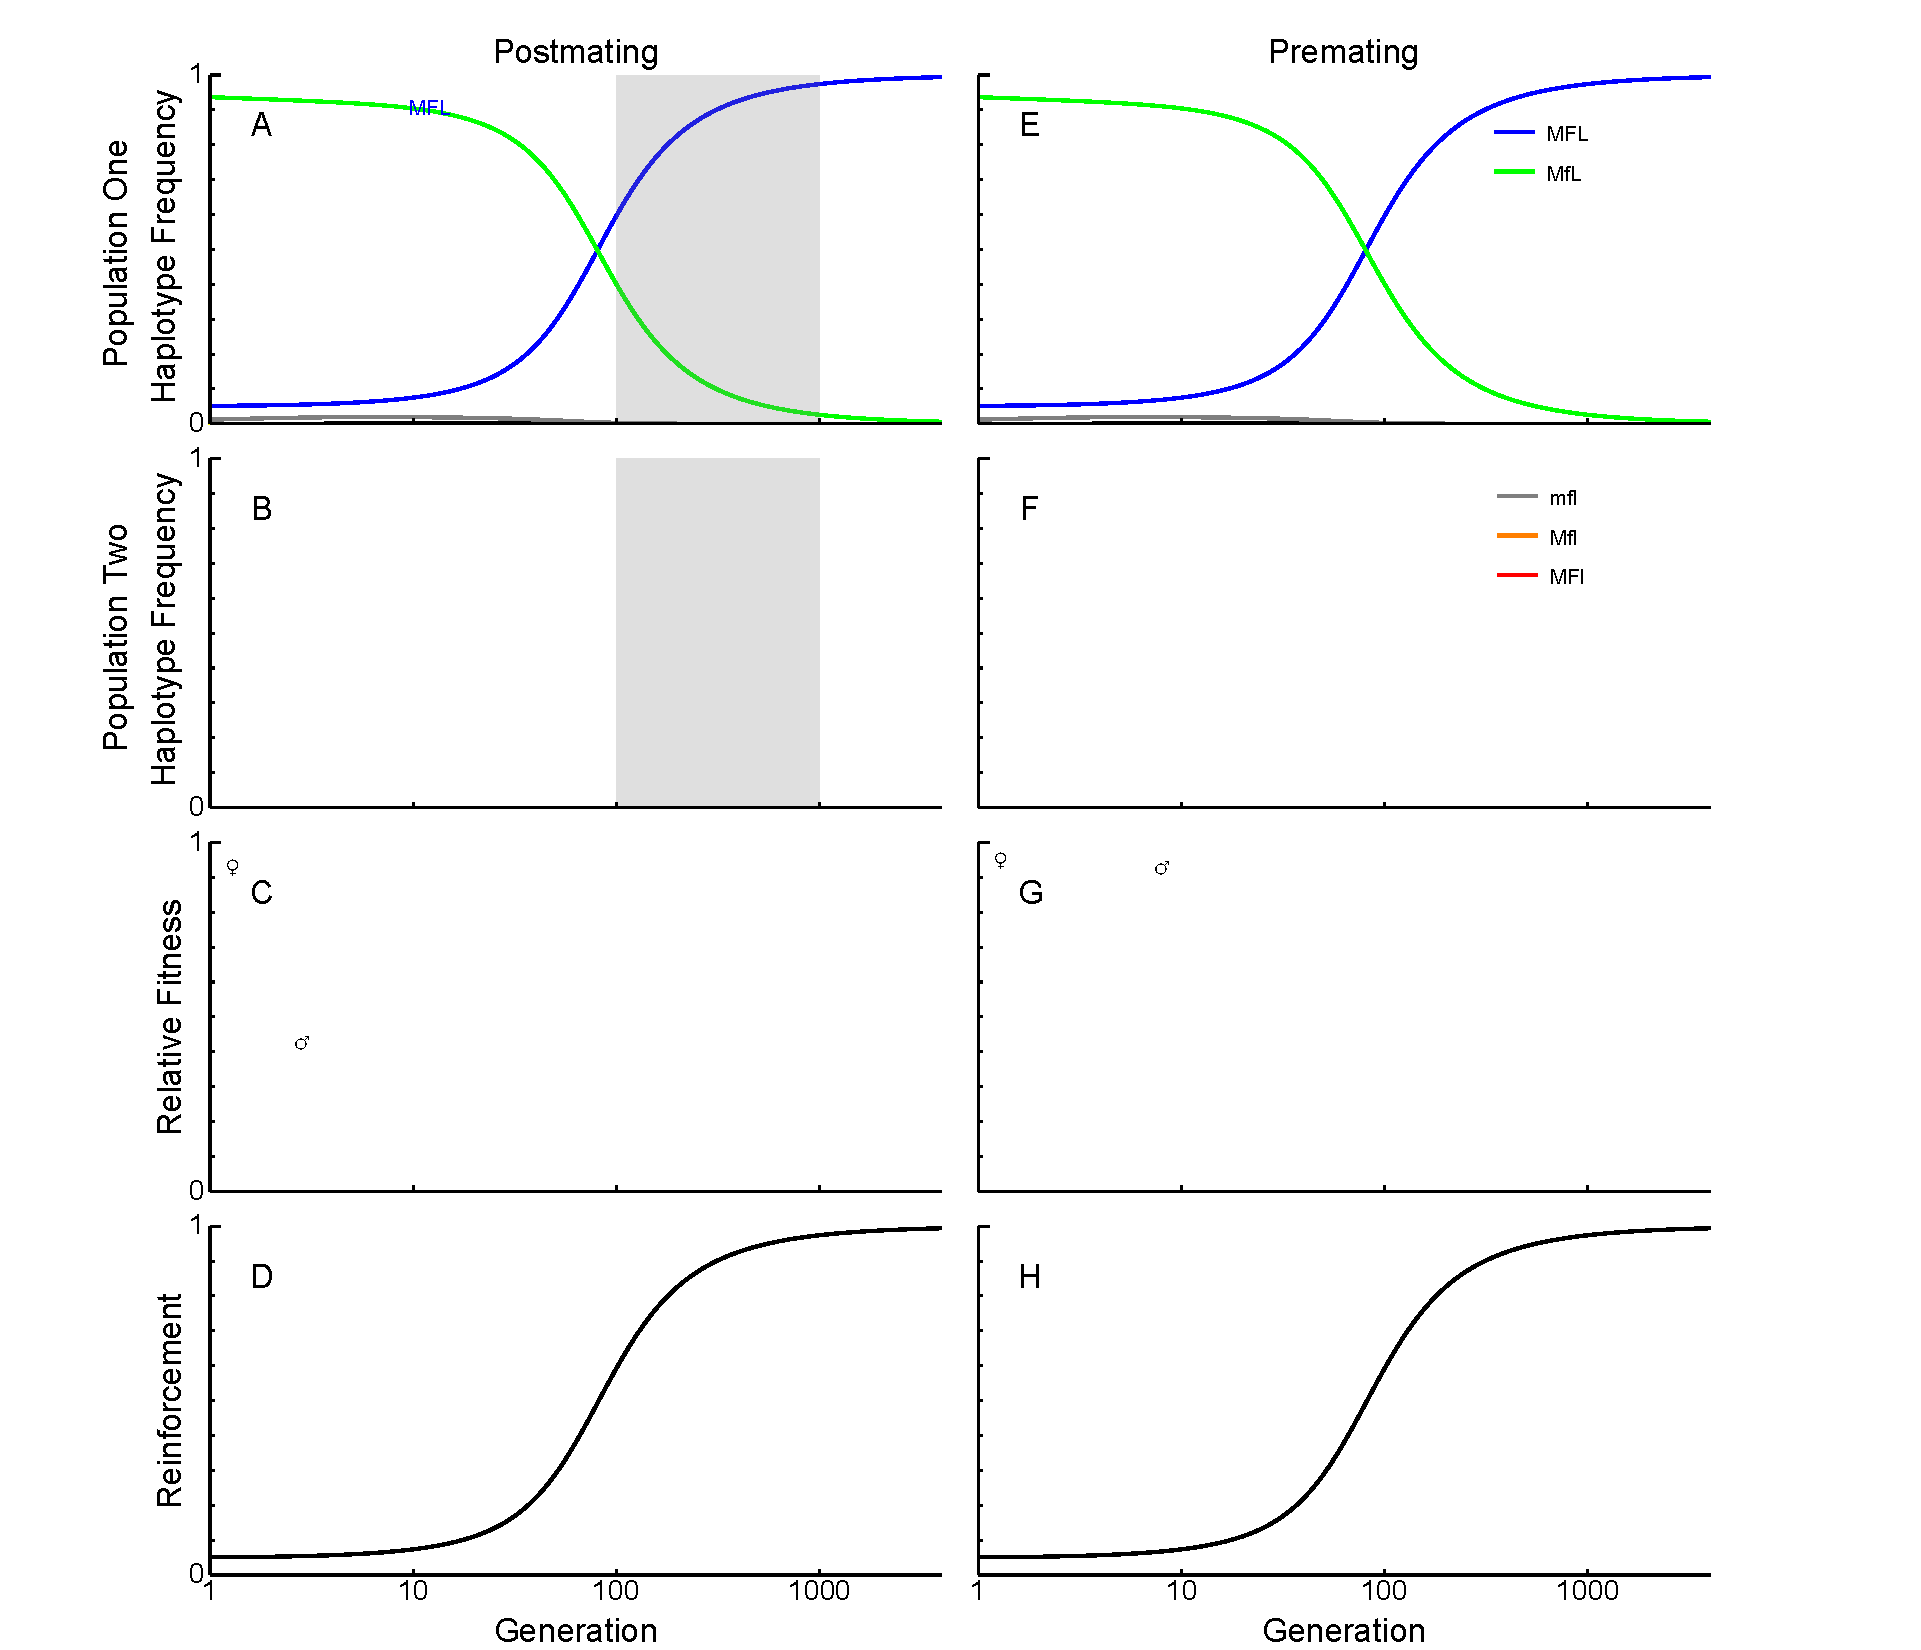
\includegraphics[width=1\textwidth]{sampleSimulations.pdf}}
\caption{
\linespread{1.618}\selectfont
Recursions over time for the postmating (A-D) and premating (E-H) model. (A) and (E) show the increase in the frequency of the barrier $F_1$ in population one.  Simultaneously, the break $M_1$ increases in frequency in population two when the barrier is postmating (B) but not when the barrier is premating (F). Thus, reinforcement in the postmating model reaches some maximum before declining to zero (C), while reproductive isolation evolves to completion in the premating model (G). In the postmating model, female fitness is higher than male fitness until the break allele has fixed in population two (CD), at which point male fitness is maximized and males `win' the sexual conflict over hybridization rate.  In the premating model, male fitness is much lower than female fitness until the barrier $F_1$ is fixed (H), at which point males from population two effectively do no migrate and only mate with conspecific females in population two.  Parameter values are $m = 0.1$, $s = 0.5$, $r_{MF} = 0$, $r_{FL} = 0.01$.}
\label{fig:sample}
\end{figure}

\FloatBarrier

\subsection*{High gene flow prevents the evolution of reproductive isolation}\label{section:migration}

Regardless of the migration rate, sexual conflict always leads to transient reinforcement. Migration rates do, however, alter speciation dynamics by changing how long reproductive isolation is non-zero and the maximum effectiveness of the isolating barrier.  For example, intermediate migration rates select for higher maximum levels of reproductive isolation than low or high migration rates (when migration is symmetric; blue lines, Fig. \ref{fig:migration}A). The evolution of reproductive isolation is limited at low migration mates because fewer maladapted hybrids are formed, exerting less selection on the barrier to increase in frequency. In contrast, high migration rates strongly select for the barrier but also increase the rate at which surviving hybrid genotypes carrying $Mf\ell$ migrate back and promote fixation of the break allele.  This decreases the number of generations where the barrier is effective (not shown). Asymmetric migration rates give further insight into the speciation dynamics by isolating the effect of changing migration in one direction. In this case it is useful to talk about the results from the perspective of a focal population (e.g., population one, but the results are analogous for population two if chosen as the focal population). Higher migration rates out of population one (i.e., high $\eta_{12}$) reduce reinforcement evolution by increasing the rate of migration of $M$-carrying genotypes to population two. When the compatibility allele spreads quickly into population two, it reduces the maximum level of reproductive isolation that can evolve before $M$ fixes and the barrier in population one is ineffective (compare the black line ($m_{12}  = 0.5$) in Fig. \ref{fig:migration}A to the red line ($m_{12} = 0.1$)). In comparison, increasing migration into population one (i.e., increasing $m_{21}$) selects for higher levels of maximum reproductive isolation (unless $m_{12}$ is also high) because the formation of many hybrids strongly favours the barrier. 

\textcolor{red}{justify asymmetrical migration Kay (2006) from Kay and Schemske (2008)}


Migration rates, whether symmetric or asymmetric, do not qualitatively affect the outcome of reinforcement for a premating barrier (when selection against hybrids is strong and recombination rates are low).  They do however, affect the rate of speciation because realized migration rates in the premating model vary over time with genotype frequency. Ignoring barrier effects on the second chromosome (for ease of understanding), $M$-carrying males will migrate at $m_{21\text{max}}$ regardless of the frequency of the barrier in population one. $m$-carrying males will migrate at a rate close to $m_{21\text{max}}$ when the barrier is rare, but will effectively not migrate when the barrier is fixed. Selection for the barrier is therefore strongest when it is rare and decreases when the barrier is common. Thus, higher maximum migration rates select for a rapid increase in the barrier, while lower maximum migration rates select for slow sustained increases in the barrier, both resulting in fixation and 100\% reproductive isolation at equilibrium.  


\begin{figure}
[!htb]
\centering
\subfloat{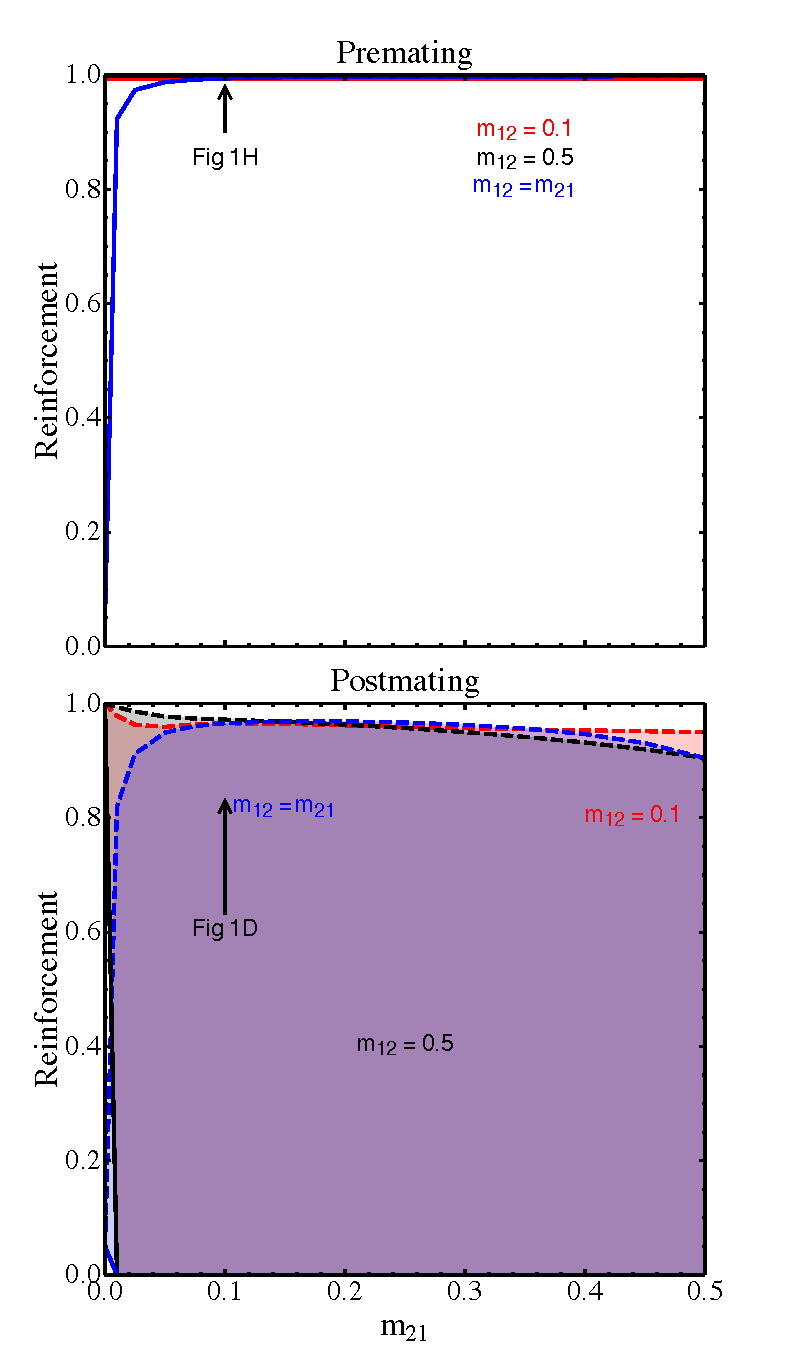
\includegraphics[width=0.5\textwidth]{migration.pdf}}
\caption{
\linespread{1.618}\selectfont
Reinforcement that evolves in population one for a postmating barrier (top panel) and a premating barrier (bottom panel), plotted as a function of the maximum migration rate, $m_{21\text{max}}$. Dashed lines represent the maximum level of reinforcement that evolved, while solid lines represent equilibrium reinforcement.  The shaded area is an indicator of the difference between maximum and equilibrium reinforcement levels. Parameter values: $r_{MF} = 0$, $r_{FL} = 0.01$, and $s = 0.5$. Note that for a premating barrier, maximum and equilibrium reinforcement are the same, and for a postmating prezygotic barrier, reinforcement always evolves to be zero at equilibrium because the break allele spreads to fixation in the other population (population two). Results are analogous for reinforcement levels in population two plotted as a function of maximum migration rate into population two ($m_{12\text{max}}$).
}
\label{fig:migration}
\end{figure}

\FloatBarrier

\subsection*{Selection}\label{section:selection}

Increasing selection against hybrid offspring (in either population) increases selection for the isolating barrier. In the postmating model, we observe higher maximum levels of reproductive isolation evolving before the barrier is rendered ineffective by the fixation of the break allele in the non-focal population (Fig. \ref{fig:selection}A).  In the premating model, complete reproductive isolation evolves when selection against hybrids is strong in both populations (Fig. \ref{fig:selection}B).  Weak selection, however, can lead to transient reinforcement.  Weak selection against hybrids in the focal population (population one) does not exert strong enough selection pressure on the barrier to increase in frequency.  Less intuitively, weak selection in population two can prevent reinforcement even when selection is very strong in population one (gray lines, Fig. \ref{fig:selection}B).  Hybrid offspring in population two survive at relatively high rates when selection is weak (e.g., $s_2 = 0.1$ in Fig. \ref{fig:selection}\textcolor{red}{B}). These hybrids are either $MfL_2$ males (that can fertilize any female in population two) or $mfL_2$ males (that can fertilize most females in population two when the barrier $F_2$ is rare).  Both carry the $M_1$ allele because it is fixed in population one. $M_1$ spreads in population two despite the fitness advantage of $m_1$-carrying males in the premating model.  The rapid spread of the break allele prevents the barrier from reaching high frequency in the focal population and makes it ineffective at preventing hybridization with population two in the long term.   



\begin{figure}
[!htb]
\centering
\subfloat{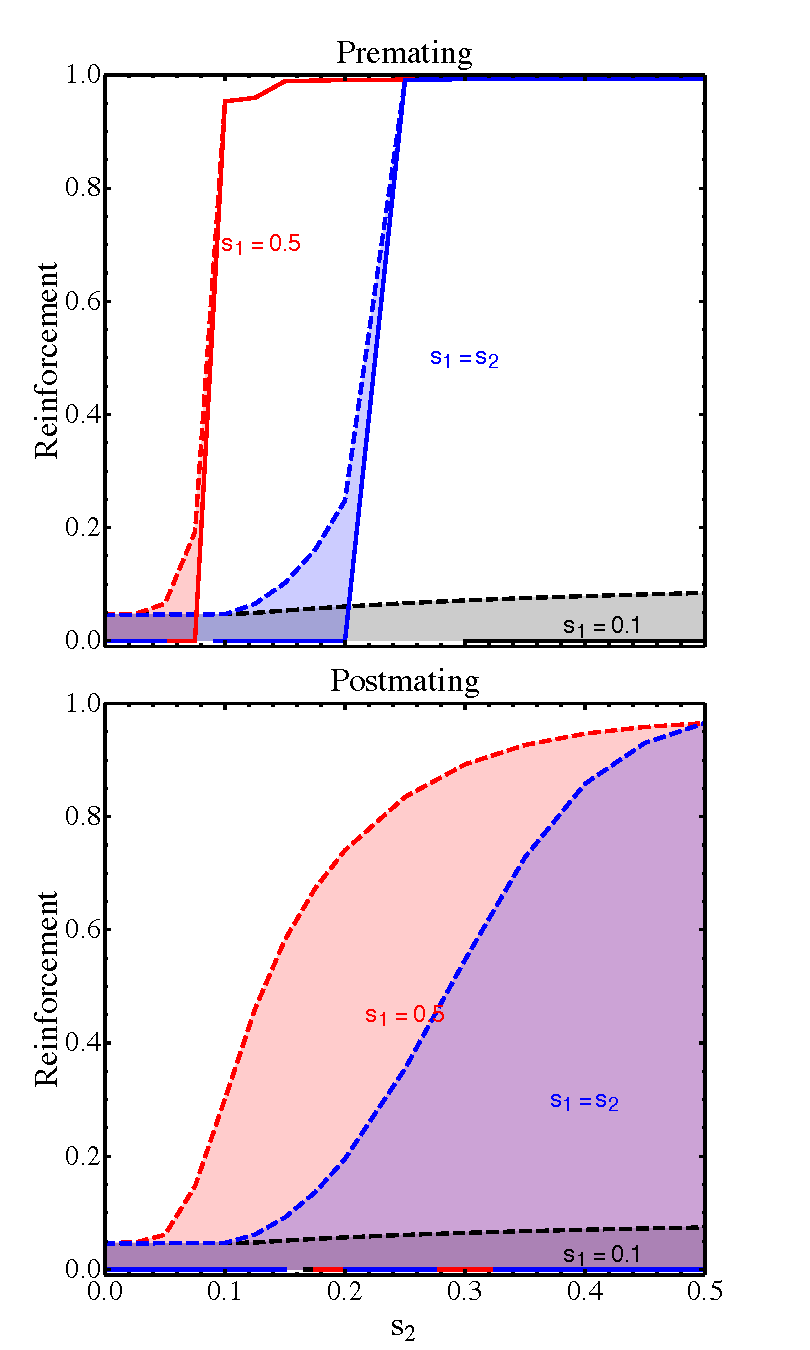
\includegraphics[width=0.5\textwidth]{selection.pdf}}
\caption{
\linespread{1.618}\selectfont
Reinforcement that evolves in population one for a postmating barrier (top panel) and a premating barrier (bottom panel), plotted as a function of selection strength against maladaptive alleles in population two, $s_{2}$. Dashed lines represent the maximum level of reinforcement that evolved, while solid lines represent equilibrium reinforcement.  The shaded area is an indicator of the difference between maximum and equilibrium reinforcement levels. Parameter values: $r_{MF} = 0$, $r_{FL} = 0.01$, and $m_{12} = m_{21} = 0.1$. Results are analogous for reinforcement levels in population two plotted as a function of selection strength against maladaptive alleles in population one, $s_1$.}
\label{fig:selection}
\end{figure}

\FloatBarrier

\subsection*{Recombination}\label{section:recomb}
\textcolor{red}{I somehow need to indicate on the figure which lines belong to the MFL model and which to the FML model}

Recombination is a well-recognized hurdle to the evolution of species boundaries because assortative mating loci must be associated with adaptive combinations of loci or locally adapted loci to ensure beneficial mate discrimination. Consistent with previous results, we find that recombination can prevent or limit the evolution of reproductive isolation. The extent to which it does so depends on the ordering of loci and the model (postmating versus premating).  \sout{In general, linkage between $M$ and $L$ is more important for reinforcement in the postmating model, while linkage between $F$ and $L$ is more important in the premating model.  }
%Thus, recombination rates have different consequences for the two models depending on the order of the loci ($MFL$ versus $FML$). 

\subsubsection*{Postmating}

 The initially rare barrier, expressed in females, relies on the genetic association between \textbf{M} and \textbf{L} across populations to ensure accepting $M$-carrying male gametes means offspring will have the local adaptation allele. Using the compatibility allele ($M$) as an indicator of conspecifics is effective until it increases in frequency in the non-focal population, which occurs via two mechanisms. Initially, $M_1$ is introduced into population two by migration and hybridization; \textit{\texorpdfstring{MfL\textsubscript{1}}{MfL 1}} (or \textit{\texorpdfstring{fML\textsubscript{1}}{fML 1}}) males fertilize females ($mf\ell_1$ or $fm\ell_1$) in population two. $M_1$ can become associated with $\ell$ in population two via recombination. Higher recombination rates facilitate introgression of the compatibility allele onto the population two genetic background. Once present in population two, it can also increase in frequency via hybridization with population one females and subsequent back migration. 
 
The introgression rate of the compatibility allele ($M$) depends on the strength of the genetic association between \textbf{M} and \textbf{L} across populations. This genetic association is broken down by two recombination rates, $r_{MF}$ and $r_{FL}$. Low $r_{MF}$ limits the spread of the compatibility allele to hybridization and back migration of rarely formed $Mf\ell$ genotypes. High $r_{MF}$ facilitates the spread of the compatibility allele by regularly creating new $Mf\ell$ genotypes. 

Free recombination When there is free recombination between the barrier ($F$) and the local adaptation allele ($L$), the compatibility allele cannot stay linked to  Recombination rates modulate the strength of the genetic association between \textbf{M} and \textbf{L} introgression of the compatibility allele onto the other species' genetic background

When \textbf{F} and \textbf{L} are tightly linked (Fig. \ref{fig:recombination}C black line, $r_{FL}$ = 0.01) reproductive isolation evolves faster and to higher maximums than if there is free recombination between them (Fig. \ref{fig:recombination}C grey line, $r_{FL}$ = 0.5). The maximum is determined by the rate of spread of the compatibility allele.


MFL - FL 0.5, assoc between M and F already 0.5
MFL - FL 0.01, as rMF increases, increases separation of M and L, lower maximums - why doesn't it get down to same as when rFL = 0.5

 Finally, recombination can give rise to genotypes carrying the barrier  and the population two local adaptation allele (i.e., $F$ and $\ell$). Once created, these $F$-carrying genotypes directly select for the compatibility allele in population two by giving it a reproductive advantage with conspecific females. If not continuously created while the compatibility allele is still spreading, genotypes carrying the barrier will disappear because \textcolor{red}{there is no selective advantage in population two.} 

\textcolor{red}{Make distinction between sexual conflict mechanisms and intraspecific reproductive advantage}
The strength of the genetic association between \textbf{M} and \textbf{L} across populations depends on recombination rates. When \textbf{F} and \textbf{L} are tightly linked (Fig. \ref{fig:recombination}C black line, $r_{FL}$ = 0.01) reproductive isolation evolves faster and to higher maximums than if there is free recombination between them (Fig. \ref{fig:recombination}C grey line, $r_{FL}$ = 0.5). The maximum is determined by the rate of spread of the compatibility allele.   Low $r_{MF}$ limits the spread of the compatibility allele to hybridization and back migration of rarely formed $Mf\ell$ genotypes. High $r_{MF}$ facilitates the spread of the compatibility allele by regularly creating new $Mf\ell$ genotypes. Changing the order of the loci does not qualitatively effect the evolution of reproductive isolation (Fig. \ref{fig:recombination}D)

%The maximum is determined by the rate of spread of the compatibility allele. The compatibility allele spreads more quickly in population two when $F$ and $L$ are unlinked because this allows the barrier to become associated with $\ell$. A barrier on the population two genetic background is not selected against and gives the compatibility allele a reproductive advantage within population two. In this case, the recombination rate between \textbf{M} and \textbf{F} does not significantly change the dynamics. In comparison, when \textbf{F} and \textbf{L} are tightly linked, maximum reproductive isolation is modulated by $r_{MF}$ (Fig. \ref{fig:recombination}C black line). Low $r_{MF}$ limits the spread of the compatibility allele to hybridization and back migration of rarely formed $Mf\ell$ genotypes. High $r_{MF}$ facilitates the spread of the compatibility allele by regularly creating new $Mf\ell$ genotypes. Changing the order of the loci does not qualitatively effect the evolution of reproductive isolation (Fig. \ref{fig:recombination}D)

and the order of the loci. When \textbf{F} and \textbf{L} are adjacent and tightly linked (Fig. \ref{fig:recombination}C black line), reproductive isolation evolves to higher maximums than if there is free recombination between them (Fig. \ref{fig:recombination}C grey line). The maximum is determined by the rate of spread of the compatibility allele. The compatibility allele spreads more quickly in population two when $F$ and $L$ are unlinked because this allows the barrier to become associated with $\ell$. A barrier on the population two genetic background is not selected against and gives the compatibility allele a reproductive advantage within population two. In this case, the recombination rate between \textbf{M} and \textbf{F} does not significantly change the dynamics. In comparison, when \textbf{F} and \textbf{L} are tightly linked, maximum reproductive isolation is modulated by $r_{MF}$ (Fig. \ref{fig:recombination}C black line). Low $r_{MF}$ limits the spread of the compatibility allele to hybridization and back migration of rarely formed $Mf\ell$ genotypes. High $r_{MF}$ facilitates the spread of the compatibility allele by regularly creating new $Mf\ell$ genotypes. Changing the order of the loci does not qualitatively effect the evolution of reproductive isolation (Fig. \ref{fig:recombination}D)



\subsubsection*{Premating}

- really takes off before the barrier spreads
-only spreads when FL is very high
- see increase and then decrease also when MF is high 
-increases at a faster rate once barrier had increased in frequency a little
-spreads inititally if the genetic assocition between M and L is broken, high recombinat between M and FL or high recombination between F and L (what is the cutoff?)
-only get introgression when rFL is very very high
MFL 
high rMF, get M briefly in population two
very high rFL, no reproductive isolation == M can only be associated with l be becoming Mfl, less likely to do that because MFL * mfl gives a lot more MFl gentoytpes , F not favoured in population two, won't get many matings

high rFL, get introgression of M regardless of rMF
high rMF, get introgression of M if rFL is also high, Mfl genotypes created and increase in frequnecy but don't take off unless MFl genotypes created
M increases first


rMF is 0.5 and rFL is 0, repro isolation evolves
In the premating model, whether reproductive isolation evolves to completion depends on whether the compatibility allele introgresses into population two. Recall that as the barrier increases in frequency in population one, only $M$-carrying males from population two can successfully mate with heterospecifics. Initially, $MfL$ males mate with $mf\ell$ females. If there is only recombination between $M$ and $F$, you get $Mf\ell$ genotypes. $M$ increases in frequency but does not take off because it has no selective advantage and the introduction of new compatibility alleles slows as the F2 barrier starts increasing in frequency. F is tied to L. Recombination between $F$ and $L$ faciliates introgression of the compatibility allele. Even if there is no recombination between $M$ and $F$, $Mf\ell$ genotypes are formed, followed by $MF\ell$., which facilities the spread and fixation of the compatibility allele.

The barrier starts increasing in frequency in population 1, but F can never be separated from L so F never increases in frequency in population two. If there is only recombination between $F$ and $L$, $MfL$ genotypes mate with $mf\ell$ genotypes. $Mf\ell$ is also created. Barrier starts increasing in frequency in population one, such that $MF\ell$ types are now created, this directly selects for $M$ in population two and reproductive isolation breaks down. rFL must be very high (greater than ??) for reproductive isolation to break down, but get break down if rMF is 0.5 and rFL is relatively high. Happens slower. But if rFL gets too low, not creating $MF\ell$ fast enough, population two barrier increases in population 2 and prevents fertilization by population 1 males carrying the population one barrier required for recombination. (DOES THIS SEEM RIGHT?)

TOMORROW  - SET RUNNING.
POLISH ALL FIGS


  $M$ increases in frequency. Once $MF\ell$ arises. and recombination between \textbf{M} and \textbf{F} allows $M$ to increase in frequency in population two via $Mf\ell$

$m$-carrying males effectively `return' to their home population and mate with conspecific $mf\ell$ females. If \textbf{F} and \textbf{L} are tightly linked, reinforcement evolves as the barrier increases in frequency in population one while the compatibility allele decreases in frequency in population two because $m$-carrying males have higher fitness than $M$-carrying males. However, if \textbf{F} and \textbf{L} are not tightly linked, the barrier can easily recombine onto the population two genetic background. Once the barrier is present in population two, the compatibility allele has a reproductive advantage with conspecific females that allows it to spread to fixation. 

Linkage between \textbf{F} and \textbf{L} depends on recombination rates and the order of the loci. If \textbf{F} and \textbf{L} are adjacent and tightly linked, permanent reproductive isolation evolves (Fig. \ref{fig:recombination}A black line). In contrast, free recombination between \textbf{F} and \textbf{L} allows the barrier to become associated with the population two local adaption allele (Fig. \ref{fig:recombination}A grey line), which gives the compatibility allele the intraspecific reproductive advantage necessary to spread. Note that it is introgression of the barrier, not sexual conflict, that prevents the evolution of reinforcement in the premating model (similar to Servedio and Burger 2014).  

If \textbf{M} and \textbf{L} are adjacent, introgression of the barrier is facilitated by increased genetic distance between $F$ and $L$. Permanent reproductive isolation is only possible if $F$ is tightly linked to $L$ through $M$. Thus, even if the compatibility and local adaptation allele are strongly linked, free recombination between $F$ and $M$ allows the barrier to recombine with $-M\ell$ to create $FM\ell$ genotypes in population two (Fig. \ref{fig:recombination}B blue line). Any recombination between $M$ and $L$ further unlinks the barrier from the local adaptation allele.




\begin{figure}
[!htb]
\centering
\subfloat{\includegraphics[width=1\textwidth]{recombination2.pdf}}
\caption{
\linespread{1.618}\selectfont
Reinforcement that evolves in population one for a premating barrier (top panels) and a postmating barrier (bottom panels).  (A and C) The MFL (black and gray) is plotted as an increasing function of $r_{MF}$, while the FML model (red and blue) is plotted as an increasing function of $r_{FM}$.  (B and D) The MFL is plotted as an increasing function of $r_{FL}$, while the FML model is plotted as an increasing function of $r_{ML}$. Dashed lines represent the maximum level of reinforcement that evolved, while solid lines represent equilibrium reinforcement.  The shaded area is an indicator of the difference between maximum and equilibrium reinforcement levels. Parameter values: $s_{1} = s_{2} = 0.5$, and $m_{12} = m_{21} = 0.1$. Results are analogous for population two. *Add note about when reinforcement goes to zero
}
\label{fig:recombination}
\end{figure}


\FloatBarrier


\subsection*{Barrier Strength}

%Reducing barrier strength intuitively decreases the amount of reinforcement that evolves.  Even if the barrier is fixed in one population and the $m$ allele is fixed in the other population, reinforcement can only be as strong as the strength of the barrier allele in preventing fertilization.  However, reducing barrier strength changes the genotype frequency dynamics.  The barrier is more likely to fix as females are selected to reduce conflict and the break allele $M$ has less advantage over $m$ and is less strongly selected for.   This means that the amount of reinforcement that does evolve is not that different from the case where the barrier is full strenght.

%-seed dispsersal
%-Felsenstein
%-

ASYMMETRICAL REPRODUCTIVE ISOLATION AND PARTIAL BARRIERS
-Tiffin et al (2001)


\section*{Discussion}

We show that sexual conflict can erode reinforced interspecific isolating barriers. 
Ever since Felsenstein (CITE) identified that recombination presents  a fundamental challenge to the reinforcement of reproductive isolation, a large body of theory has aimed to identify how and when reinforcement could evolve (CITE  LOADS). 
Consequently, the identification of further theoretical challenges to the evolution of reinforcement has lagged (but see Servedio for an important counterexample).

Despite, or perhaps because of, its role in hampering speciation, sexual conflict over hybridization has received little attention in the literature \citep[but see ][]{Parker1998, Parker and Partridge, Gavrilets}.  
% since the idea was first proposed in a game theoretic framework twenty years ago \citep{Parker1998}. 
%While previous work \citep{Parker1998, Gavrilets2014} highlighted the possibility of interspecific sexual conflict and speculated on its macroevolutionary consequences, it did not generate the population genetic predictions necessary to identify if such a conflict has occurred or is occurring. 
Our population genetic analysis shows the transient dynamics generated by sexual conflict over reinforcement and the genetic signatures it leaves behind. 
The results provide a rich set of predictions and interpretations of empirical patterns that were missed by previous game theoretic \citep{parkerpartridge, gavrilets} and verbal \citep{Coyne} descriptions of the potential for such conflicts. 
We show that interspecific sexual conflict favors male gametic traits that overcome heterospecific female barriers. 
Beleaguered by interspecific sexual conflict, the break down of reproductive isolation is marked by the rapid adaptive introgression of male compatibility factors, followed by the slow homogenization of the frequency of female barriers across species. 
By contrast, in the absence of such conflict, species-specific compatibility alleles  cross species boundaries under a more restricted set of parameters.
Ultimately, we show that barriers acting at different stages of hybridization can affect how reinforcement proceeds.
%The rate and pattern of introgression in models with and without sexual conflict depends on the strength of other evolutionary forces. \textcolor{red}{say instead: no sexual conflict, results no different than classic reinforcement model?}
%We show that barriers acting at different stages of hybridization can affect how reinforcement proceeds.

\paragraph{Sexual conflict over the reinforcement of  pre- and post-mating barriers:}    
To isolate the role of sexual conflict in preventing reinforcement, we compared models of the reinforcement of pre- and post-mating barriers, representing  the absence and presence of sexual conflict, respectively.  
In our model, males can redirect their reproductive efforts towards conspecific females if rejected by a premating barrier. 
However, because males faced with a postmating-prezygotic barrier are rejected after mating, their gametes lose the opportunity to fertilize conspecific females. 
%have higher fitness if sperm fertilize heterospecific eggs. 
%For example, in the face of an interspecific difference in flowering times of a dioecious plant, male fitness will increase as a greater proportion of  pollen is available for its conspecific styles. 
%However, once pollen has landed on a (potentially heterospecific) pistil male fitness can only increase if fertilization is successful.  
%Populations potentially separated by a postmating prezygotic barrier will inherently face sexual conflict over the hybridization rate (in the absence of mate limitation, search costs, or other costs that may favour hybridization in the choosy sex).  
Thus, a conflict arises in the postmating case because females are selected to avoid hybridizing while male gametes are selected to overcome the opportunity cost associated with no longer having the option to fertilize conspecific females.  
This conflict is borne out in our population genetic models. 
Following the initial increase in frequency of distinct postmating-prezygotic isolating barriers in each population, complementary male compatibility alleles adaptively introgress  into heterospecific populations.  
Reproductive isolation eventually disappears, as the fixation of previously species-specific compatibility alleles renders the isolating barriers ineffective.

By contrast, premating barriers can be stably reinforced under a much broader range of parameter space. 
As modeled in our work, a premating barrier alleviates sexual conflict by giving rejected males the opportunity to mate with compatible conspecific females.  
As such, migrated males that successfully mate with heterospecific females have lower fitness than rejected males, who subsequently succeed in intraspecific mating. 
This aligns selection on male and female hybridization rates, making the evolution of reinforcement much more plausible. %, as  males that successfully mate with heterospecific females have lower fitness than rejected males, aligning selection on male and female hybridization rates. 
We note that, while our model of prezygotic isolation is quite specific, its key feature --- that by mating with heterospecifics, males miss opportunities to mate with conspecifics --- is implicit in most one and two- allele models of reinforcement (see ``Comparison to Previous Models'', below). 
However, the differences in the biology underlying these premating barriers will result in quantitative differences between our premating model and previous results. 


We believe that sexual conflict over reinforcement is more likely for postmating than for premating barriers. 
However, this mapping is not absolute and will depend on details of the biological system.   
%\textcolor{red}{That is, there are likely scenarios in which the fitness benefit of siring a low-fitness hybrid outweighs the opportunity cost of a heterospecific mating opportunity \cite{Parkerpartidge}.}  \textcolor{blue}{Take for example, flowering time, if the survival of maladaptive hybrids outweighs the fitness cost of shedding pollen on days when heterospecific, but not conspecific styles are receptive, selection will favor extending  male flowering  time.} \textcolor{red}{YANIV I DON'T UNDERSTAND THIS SENTENCE} \textcolor{blue}{did this example help? I like this sentence and think it's important.}
That is, certain physical and/or biochemical properties of postmating interactions can minimize the opportunity for interspecific sexual conflict by enforcing a trade-off between overcoming a heterospecific barrier and successfully fertilizing conspecifics.    
For example, if pollen must travel far enough, but not too far, down the style to achieve fertilization \citep[as observed in interspecific crosses in Nicotiana ][]{Lee2008}, pollen will not be able to simultaneously succeed on both inter- and intra- specific styles.
This will minimize the opportunity for interspecific sexual conflict.  
Indeed, a change in style length appears to underlie the evolution of reinforcement in a sympatric \textit{Silene} species pair \citep{Nista2015}.  
More directly, in competitive fertilization, factors modulating intraspecific gamete precedence provide mechanisms by which the reinforcement of postmating-prezygotic barriers may stably evolve \citep{Howard199,Lorch2007}.   
As such, the observation that conspecific sperm precedence is reinforced in sympatric populations of \citep{Drosophila pseudoobscura}  and \citep{D. persimilis} \citep{Castillo_biorXiv} is broadly consistent with our theory.  



%Reproductive isolation eventually evolves to zero as the fixation of previously species-specific compatibility alleles renders the isolating barriers ineffective. 
%The transient reinforcement of a postmating prezygotic barrier is observed for all parameter values studied here (with the exception of \textcolor{red}{extreme asymmetrical migration}). 

%For a premating barrier (no conflict), the strength of selection affects whether reprodctive isolation is permanent or transient. Weak selection reduces selection on the barrier such that increases in frequency slowly enough for some hybrids to be formed. Formation of an appreciable number of hybrids at migration selection balance allow the barriers to introgress into the other populations, which then selects for the compatbility allele directly and prevents reproduction from evolving.

%In contrast, a premating barrier gives rise to equilibrium reproductive isolation unless the barrier itself introgresses. A premating barrier alleviates sexual conflict by giving rejected males the opportunity to mate with compatible conspecific females. Reproductive isolation evolves because migrated males that successfully mate with heterospecific females have lower fitness than rejected males, aligning selection on male and female hybridization rates. When permanent reproductive isolation does not evolve in the premating model, it is because selection against hybrids is not strong enough to overcome migration or because recombination breaks up the barrier and local adaptation locus. In either case, the barrier introgresses into the other population and selects for its own species-specific compatibility allele.  
%Thus, even in our premating model we see transient reproductive isolation across more areas of parameter space than previous reinforcement models.
%the qualitative outcome depends on three evolutionary forces: selection, migration, and recombination.EXPAND? BRIEFLY MENTION PARAMETERS
%BUT STILL SEE REINFORCEMENT LESS THAN OTHER MODELS. WHY?


%\sout{When permanent reproductive isolation does not evolve in the premating model, it is because selection against hybrids is not strong enough to overcome migration or because recombination breaks up the barrier and local adaptation locus. In either case, the barrier introgresses into the other population and selects for its own species-specific compatibility allele.}  

\paragraph{Comparison to previous models:}  
The mechanism of assortative mating is a major distinguishing feature of our reinforcement model. 
In our model, a female expressed isolating barrier requires a male expressed compatibility allele to overcome it.   % yb deleted (whether postmating-prezygotic or premating)
Introgression of this male compatibility allele is facilitated by the fact that it does not prevent mating with conspecifics. 
This \textit{lock/key} model of reproductive isolation was inspired by the mechanism underlying well-understood cases of postmating isolation (CITE maize/teo, sea urchin, and abalone). 
For example, pollen-style (in)compatibilities between \textit{Zea mays} subspecies are controlled by pairs of loci known as gametophytic factors, for which stylar rejection phenotypes are overcome by the expression of pollen compatibility alleles at a tightly linked locus \cite{NELSON,1993}. 
%, including the gametophytic factor system in \emph{Z. maize} spp. (CITE), the bindin/EBR1 system in sea urchins (CITE), and the lysin/VERL system (CITE) in abalone. 
By contrast, previous reinforcement models incorporating separate sexes typically treat the sexes interchangeably \citep[e.g. ][]{Felsenstein}, or assume assortative mating by a female preferences for diverged male traits (Lande PNAS, Servedio and Kirkpatrick 1997, Kelly and Noor... others?). 
These \textit{preference/trait} models implicitly induce a trade-off between interspecific and intraspecific mating --a male with a trait favored by heterospecific females will have limited mating success with conspecifics. 
As such, while \textit{lock/key} type of mating interactions can result in the transient -- and ultimately failed -- reinforcement of postmating-prezygotic isolation, this outcome does not arise in \textit{preference/trait}  type models.%  \textcolor{red}{SHOULD WE MENTION COSTUS SPP.?} \textcolor{blue}{ NOOOOOO}

%The mechanism of assortative mating is a major distinguishing feature of our model of sexual conflict over reinforcement. Most previous reinforcement theory that allows for separate sexes models premating barriers as female preferences for diverging male traits (Lande PNAS, Servedio and Kirkpatrick 1997, Kelly and Noor... others?). If males of one species evolve the preferred trait of the other, they do so at the expense of intraspecific mating opportunities. Classic preference/trait models therefore induce a trade-off between interspecific and intraspecific matings \sout{that make the evolution of reproductive isolation more likely than either of our models}. In comparison, we assume an isolating barrier (whether postmating [prezygotic] or premating) that requires a compatibility allele to overcome it. Introgression of species-specific compatibility alleles is facilitated by the fact that these do no prevent mating with conspecifics. This \textit{lock and key} model of reproductive isolation was inspired by the mechanism underlying well understood cases of postmating isolation, including the gametophytic factor system in \emph{Z. maize} spp. (CITE), the bindin/EBR1 system in sea urchins (CITE), and the lysin/VERL system (CITE) in abalone and highlights the potential for an interspecific sexual conflict to result in the transient -- and ultimately failed -- reinforcement of postmating isolation. \textcolor{red}{Costus?}. 

The role of sexual conflict in removing species boundaries runs counter to the conventional role sexual conflict is thought to play in speciation  \citep[][]{GavriletsWaxman,RiceandHistert,ParkerPartrdige}. 
Previous theory \citep{GavriletsWaxman} and experiments \citep{Rice1996Nature} suggested that sexually antagonistic coevolution can lead to coevolutionary arms races in each incipient species, pleiotropically resulting in behavioral or mechanical isolation. 
In this manner \emph{intraspecific} sexual conflict was thought to be an "Engine of Speciation" \citep[e.g. ][]{RiceandHistert}.  
In contrast, interspecific sexual conflict hampers speciation by preventing the evolution of reinforcement, despite both types of conflict (intra- and interspecific) arising from male propensity to mate and female propensity to resist certain matings. 

We are not the first to show that sexual selection can act to  bring species together, rather than pushing them apart. 
Recently, Servedio and Burger's (2015) found that Fisherian sexual selection can undermine the evolution of assortative mating.
They showed that when female preference can introgress across  species backgrounds, they can favour heterospecific male traits by sexual selection even when such traits are disfavored by natural selection.   
By  providing a mating advantage to maladaptive male traits, this model undermines the evolution of reinforcement.  
In some areas of parameter space, our pre-mating model shows that the preference introgresses faster than the trait and then selects for spread of the species-specific compatibility allele, replicating the finding of Servedio and Burger (2015).  \textcolor{red}{Is this true? STILL WORKING ON FIGURING THIS OUT}  
However, the dynamics of our postmating model reveal a much different story -- a sperm's ability to overcome a reproductive barrier adaptively introgresses across species' boundaries, while the barrier allele is disfavored, and can only cross species boundaries once the sperm trait is common. \

%Our work is not  the first to suggest that sexual conflict could hinder reinforcement (see Parker and Partridge, Coyne and Orr, Gavrilets). 

%DO WE WANT TO KEEP A VERSION OF THIS PARAGRAPH
%However previous models of this process where either entirely verbal (Coyne and Orr) or game theoretic (Parker and Partridge, Gavrilets). \textcolor{red}{I THINK THAT IF WE SAY WE ARE GOING TO COMPARE OUR MODEL TO THE TWO MOST CLOSELY RELATED PAPERS WE NEED TO WRITE MAYBE TWO SENTENCES COMPARING OUR RESULTS TO THOSE OF PARKER and PARTRIDGE. Can you add this? You have a much better understanding of their paper than I do. Be careful not to same thing we say in the introduction}
%Therefore these previous models did not predict that such a conflict would, for example result in the transient evolution of reinforcement, or that it would favor the adaptive introgression of male traits across species boundaries. 

\paragraph{Predictions and interpretations of empirical data:}      
%The unexpected role of sexual conflict in removing species boundaries is counter to the conventional role sexual conflict is thought to play in speciation. 
%Previous theory has suggested that sexually antagonistic coevolution can lead to coevolutionary arms races in each incipient species such that upon secondary contact, species have diverged to the point of being behaviourally or mechanically isolated. 
%In this manner \emph{intraspecific} sexual conflict is thought to contribute to or drive speciation. 
%In contrast, interspecific sexual conflict hampers speciation by preventing the evolution of reinforcement, despite both types of conflict (intra- and interspecific) arising from male propensity to mate and female propensity to resist certain matings. 

We show that sexual conflict can result in the transient evolution of reinforcement.  
Specifically, we expect the transient reinforcement of \textit{lock and key} postmating prezygotic barriers in which males do not trade off inter- and intraspecific mating success.  
This major result -- that is, that postmating prezygotic barriers are rarely stably reinforced,  can explain numerous empirical  observations.  
Most straightforwardly, our result is consistent with the finding that postmating prezygotic isolation does not differ between sympatric and allopatric species pairs across three angiosperm genera (Moyle et al), suggesting that these barriers are not reinforced among sympatric species.
Additionally, our findings are compatible with the growing consensus that, contrary to initial claims, reinforcement does not drive the evolution of sperm-egg interactions underlying reproductive barriers in broadcast spawners (Lessios, 2007; \textcolor{red}{Palumbi and Lessios 2005; Vacquier and Swanson 2011}). 

Most immediately, our model provides a clear interpretation and novel predictions concerning patterns of geographic variation at loci underlying cross compatibility between \text{Zea mays} subspecies. 
These `Gametophytic Factors' consist of tightly linked alleles in which stylar barriers require pollen signal for effective pollination \citep{Things}, a mechanism  that inspired our modeling approach.   %The evolution of gametophytic factors in \textit{Zea mays spp.} provide an opportunity for refined tests of our theory. 
As predicted by standard models of reinforcement, styles of  the wild teosinte, \textit{Z. m. mexicana}, grown near \textit{Z. m. mays} landraces, reject most maize pollen. 
However, ``[t]he  unexpected  presence  of  the [male compatibility] allele in sympatric landrace maize appear[ed]... to negate  any  effect  of  [the] crossing  barrier" puzzling researchers \citep{medyca paper}.   %YANIV I DON"T THINK YOU NEED TO QUOTE THIS
Our model predicts that adaptive introgression of the teosinte allele is responsible for the compatibility of sympatric \textit{Zea m. mays} / \textit{Z. m. mexicana} populations.  
Isolating and sequencing compatibility haplotypes in these maize landraces will provide a strong test of our theory. 

Our results highlight an under-appreciated challenge to the reinforcement of postmating-prezygotic barriers. 
However, rather than negating our theory, cases in which  postmating-prezygotic barriers are reinforced provide a strong opportunity to further test our theory.  
We predict that cases in which postmating prezygotic isolation is reinforced should (1) be transient, (2)  entail a trade-off between male success in overcoming  inter and intraspecific postmating barriers and/or (3) involved unidirectional gene flow. 
As such, the few documented cases in which postmating-prezygotic barriers are reinforced (without conspecific gamete precedence) are of particular interest to our theory.   
We know of two such cases. 
Kay \citep{Kay and Schemske, Yost and Kay}, demonstrated that post-pollination barriers are reinforced in a pair of wild gingers. 
Importantly, however, gene flow in this species-pair is unidirectional, negating any sexual conflict over reinforcement. \textcolor{red}{Ali do we have a graph showing this?} %YANIV.. SHOWING WHAT? 
Matute (2010) convincingly found that \textit{Drosophila yakuba} females from populations sympatric with \textit{D. santomea},show elevated gametic isolation from \textit{D. santomea}, but show no evidence for conspecific sperm precedence. 
Our theory provides the strong prediction that swapping \textit{D. yakuba} male compatibility alleles into  \textit{D. santomea} males will result in less effective intraspecific matings. % I THINK THEY MAY HAVE A UNIDIRECTINAL THING GOING TOO
Thus, in addition to making sense of known observations, our model provides novel research directions.  
In sum, our work explains the paucity of well-established cases of the reinforcement of postmating prezygotic barriers, and generates specific testable predictions when these barriers appear to be reinforced. 




%We show that sexual conflict is expected to lead to the transient evolution of \textit{lock and key} postmating [prezygotic] barriers. 
%That we do not expect stable reinforcement of postmating [prezygotic] barriers seems largely consistent with observations in nature. 
%In an extensive survey of  postmating prezygotic isolation  in three angiosperm genera,  Moyle et al () found no evidence of elevated isolation in sympatry, suggesting that these barriers are not reinforced. 
%%The transient nature of reinforcement may explain why there are so few empirical examples of reinforcement evolving through a postmating prezygotic barrier. 
%Similarly, while postmating prezygotic barriers are well documented in broadcast spawners (Lessios, 2007; \textcolor{red}{Palumbi and Lessios 2005; Vacquier and Swanson 2011}) and where initially thought to reinforce species barriers (CITE), subsequent studies have largely dismissed this hypothesis (CITE). 
%%wind pollinated plants (ref). But in general thought to be low in animals and plants (Moyle et al 2004). 
%These types of barriers appear to be less common between species pairs more capable of evolving premating barriers, but have been found in animals with internal fertilization (e.g. Drosophila \citep{Matute:2010bm}) and plants that share pollinators (Kay and Schemske 2008) has documented the only known example in internalizing fertilizing animals RARE, few examples of postmating prezygotic barriers reinforcement in nature.   
%Our results suggest a novel hypothesis to explain these findings -- that is, that female barriers at eg EBR1 and VERL that reject heterospecific sperm may be initially favored in sympatry but that sperm traits encoded by  bindin and lysin that can overcome these barriers evolve to overcome these incompatibilities. 
% YANIV -- WHY ARE YOU SAYING Z. MAYS IS AN OPPORTUNITY TO TEST THIS, AND NOT DROSIPHILA OR COSTUS OR SOMETHING?

%Our theory make strong predictions in cases in which postmating barriers are reinforced (\textit{Costus scaber}/ \textit{C. pulverulentus}  and \textit{D. yakuba} / \textit{D. santomea}).  
%We predict that such cases either lack bidirectional gene flow,  are transient, or consist of physical / chemical barriers in which heteospecific fertilization success comes at the cost of conspecific success.  


\paragraph{Future Directions:}

For ease of analysis and interpretation, we made numerous additional assumptions in our reinforcement models of both pre- and postmating barriers.  
For example, we modeled postzygotic isolation by assuming that hybrids are not well adapted to either parental species' habitat (e.g., Schluter 1998), rather than assuming intrinsic hybrid incompatibility arising from a single underdominant locus or two locus Dobzhansky-Muller interactions.  
We further assumed a relatively simple basis of local (mal)adaptation -- each prezygotic incompatibility was linked to one local adaptation locus, and fitness was multiplicative both within and among locally (mal)adaptive loci. 
%and that populations exited in two simple demes rather than e.g. a more complex cline.  
Future empirical work should aim to identify model systems in which to test our hypothesis, and novel theory, involving the relaxation of these assumptions, should be tailored to the biologically-inspired scenarios investigated. 

%\sout{Additionally, we assumed a simple two deme model, rather than, for example a cline. }

%All of these outcomes are likely to change quantitative predictions of our model, but are unlikely to fully defuse the sexual conflict evaluated by our model. 
%One area of particular interest is the genetic architecture of hybrid unfitness. 
%Kirkpatrick (2001) found that reinforcement was stronger in cases where many loci contributed to ecological divergence, and in our model a sufficient density of (mal)adaptive alleles on either side of incompatibility loci could decrease the fitness gains associated with siring low fitness hybrids.  
%Future work should address how changing these assumptions qualitatively alters the impact of sexual conflict on the evolution of reinforcement - this will be especially important for cases in which theory is used to infer evolutionary parameters from population genomic data.   
%We make the assumption that such postzygotic isolation is captured by divergent selection on two local adaptation loci and that selection acts multiplicatively against maladaptive alleles. While this is certainly an oversimplification (100s of genes underly the genetic basis of local adaptation, refs), \textcolor{red}{it ensures we make conservative predictions about the likelihood of reinforcement evolution.} For example, Kirkpatrick (2001) modeled multiple loci underlying an ecolocigal trait and found that reinforcement was stronger in cases where many loci contributed to phenotype. 
%In addition to modifying the genetic basis of local adaption, future work might consider other forms of selection against hybrids that can lead to reinforcement.  The most commonly observed (ref.) and modeled (Servedio, etc) is genetic incompatibilities, also known as Dobzhanksy-Muller incompatibitilies (DMI). DMIs arise when populations have diverged in allopatry and mutant alleles have not been tested on new genetic backgrounds. Because DMIs require a minimum of two loci, modeling postzygotic isolation would require replacing a local adaptation locus with two incompatiblitiy loci. We predict a model of this type would be even less likely to evolve reproductive isolation because strong linkage disequilibrium is required to maintain selection against hybrids. 

%Alternatively, we could model hybrids with reduced reproductive success. Hybrids may be partially sterile (e.g. refs) or have lower mating success because of intermediate traits that reduce attraction of females of either parental species (Lemmon and Lemmon 2010) or reduce attraction of pollinators (Schemske and Bradshaw 1999). We expect incorporating reduced reproductive success of hybrid offspring to also reduce the likelihood of reinforcement because selection against interspecific mating is strongest if it occurs in the parental generation (e.g. Grant 1966), and decreases when selection is in subsequent generations (e.g. F1 generation: reduced hybrid viabiliy and offspring production). Alternatively, many of these postzygotic barriers may be acting simultaneously and contributing to repoductive isolation.
 

\section*{Methods}
%YANIV WE NEED A LITTLE CONTEXT FOR THIS SECTION
The genotypes on chromosome one and two are denoted by $i_1$ and $i_2$, respectively.  Genotypes on chromosome one are numbered one through eight such that $i_1 = 1, 2, 3, 4, 5, 6, 7, 8$ represents $M F L_1$, $M f L_1$, $m F L_1$, $m f L_1$, $M F \ell_1$, $M f \ell_1$, $m F \ell_1$, $m f \ell_1$, respectively. Genotypes are defined analogously for chromosome two. The genotype designation for both chromosomes is given by $X_{i_1 i_2}$.  For example, $X_{1 1}$ represents haploid genotype $M F L_1 M F L_2$.

\noindent \textbf{Migration:} Only a fraction $\eta_{kn}$ of males migrate from population $k$ to population $n$.  The remaining fraction $(1-\eta_{kn})$ do not disperse and comprise part of the mating pool in population $k$ together with the fraction of heterospecific males $\eta_{nk}$ dispersed from population $n$.  We normalize genotype frequencies by the sum of all males in a given population's mating pool so that genotype frequencies sum to one even if there is asymmetric migration.  Equation \ref{Eq:eq1} describes haploid genotype frequencies of males after migration (denoted by an $^*$) in population $k$.  

\begin{equation}\label{Eq:eq1}
X^*_{{i_1 i_2}, k} = ((1 - \eta_{kn}) X_{{i_1 i_2}, k} + \eta_{nk} X_{{i_1 i_2}, n})/ \sum_{i_1 =1}^{8} \sum_{i_2=1}^{8} ((1 - \eta_{kn}) X_{{i_1 i_2}, k} + \eta_{nk} X_{{i_1 i_2}, n})
\end{equation}

\noindent \textbf{Mating:} The probability of mating between males of type $X^*_{i_1 i_2}$ and females of type $X_{j_1 j_2}$ in population $k$ is given by

\begin{equation}\label{Eq:eq2}
M^{**}_{i_1 i_2, j_1 j_2, k} = (1 - \text{c} b_1 \text{d} b_2) X^*_{i_1 i_2, k} X_{j_1 j_2, k}/ \sum_{i_1 =1}^{8} \sum_{i_2=1}^{8} (1 - \text{c} b_1 \text{d} b_2) X^*_{i_1 i_2, k}
\end{equation}

where $\text{c} = 1$ if $j_1$ carries the $F_1$ allele and $i_1$ carries the $m_1$ allele, and $\text{c} = 0$ otherwise.  Similarly, $\text{d} = 1$ if $j_2$ carries the $F_2$ allele and $i_2$ carries the $m_2$ allele, and $\text{d} = 0$ otherwise.  $b_1$ and $b_2$ represent the barrier strength of the $F_1$ and $F_2$ alleles, respectively. A barrier strength equal to one means the barrier allele is 100\% effective at preventing mating/fertilization with males not carrying the corresponding compatibility allele.  

\noindent \textbf{Selection:} After mating, selection acts on the diploid offspring according to equation \ref{Eq:eq3}.

\begin{equation}\label{Eq:eq3}
S^{**}_{i_1 i_2, j_1 j_2, k} = (1 - s_1)^{e} (1 - s_2)^{f} M^{**}_{i_1 i_2, j_1 j_2, k}/\bar{w}
\end{equation}

where $s_1$ and $s_2$ are the strengths of selection against maladaptive alleles at locus \textbf{\texorpdfstring{L\textsubscript{1}}{L 1}} and \textbf{\texorpdfstring{L\textsubscript{2}}{L 2}}, respectively.  $e = 0$ if there are no maladaptive alleles at \textbf{\texorpdfstring{L\textsubscript{1}}{L 1}} (either from the male gamete, $i_1$, or female gamete, $j_1$), $e = 1$ if there is one $L$ allele in a population where $l$ is favoured (and vice versa), and $e = 2$ if there are two maladaptive alleles.  Selection works similarly at the local adaptation locus \textbf{\texorpdfstring{L\textsubscript{2}}{L 2}} and the two loci interact multiplicatively to determine the overall strength of selection.

\noindent \textbf{Recombination:} Diploid offspring undergo recombination and segregation to form haploid gametes following the standard algorithms. We explore a range of scenarios ranging from perfect linkage to free recombination between loci on a chromosome. 

\subsection*{Starting Genotype Frequencies} 

We assume the two (incipient) species are initially only separated by a postzygotic ecological isolating barrier (i.e. hybrid offspring are unfit).  The barrier ($F_1$ or $F_2$) in each population is rare and we investigate the evolution of reproductive isolation when a rare compatibility allele, ($M_1$ and $M_2$) arises in the other species (fig. \ref{fig:figure1}B).  Specifically, population one starts with $M F L_1 m f L_2 = 0.95$ and $M f L_1 m f L_2 = 0.05$. This means that with respect to the first set of assortative mating loci, the compatibility allele ($M_1$) is fixed and the barrier is rare ($p_{F_1} = 0.05$). At the other set of assortative mating loci, the compatibility allele is absent ($M_2 = 0$) such that initially, males could not overcome an isolating barrier in the other species if it were common.  Initial genotype frequencies in population two are analogous (i.e., $M_2$ is fixed and $F_2$ is rare, while males could not overcome am isolating barrier in population one ($M_1 = 0$). 

\subsection*{Measuring Reproductive Isolation}
%YANIV THIS PROBABLY ALSO NEEDS A LITTLE CONTEXT (IT IS REFERRED TO ABOVE IN THE "MODELING" SECTION
\begin{equation}\label{Eq:eq4}
reinf = \sum_{i_1 i_2}^{64} \sum_{j_1 j_2}^{64} (1 - \text{c} b_1 \text{d} b_2) X^*_{i_1 i_2, k} X_{j_1 j_2, k}/ \sum_{i_1 =1}^{8} \sum_{i_2=1}^{8} (1 - \text{c} b_1 \text{d} b_2) X^*_{i_1 i_2, k}
\end{equation}  

\newpage
\bibliography{speciationLibrary}
\bibliographystyle{amnatnat}


\end{document}